\chapter{Configuring a Cache-only DNS Server}

	\section{Understanding DNS}
A DNS/name server provides IP addresses for any domain name. To do this every DNS name server has a cache where it keeps the records of all the previous lookups it has done. Let us consider 3 hosts using the same name server. Let's assume initially, the cache of the host is empty, except the IP of the root name server. Now if \textit{Host 1} wants to connect to \verb|www.microsoft.com| then it'll ask for the IP to the name server. The name server tries to find it in it's cache but can't.  

\begin{figure}[H]
	\centering
	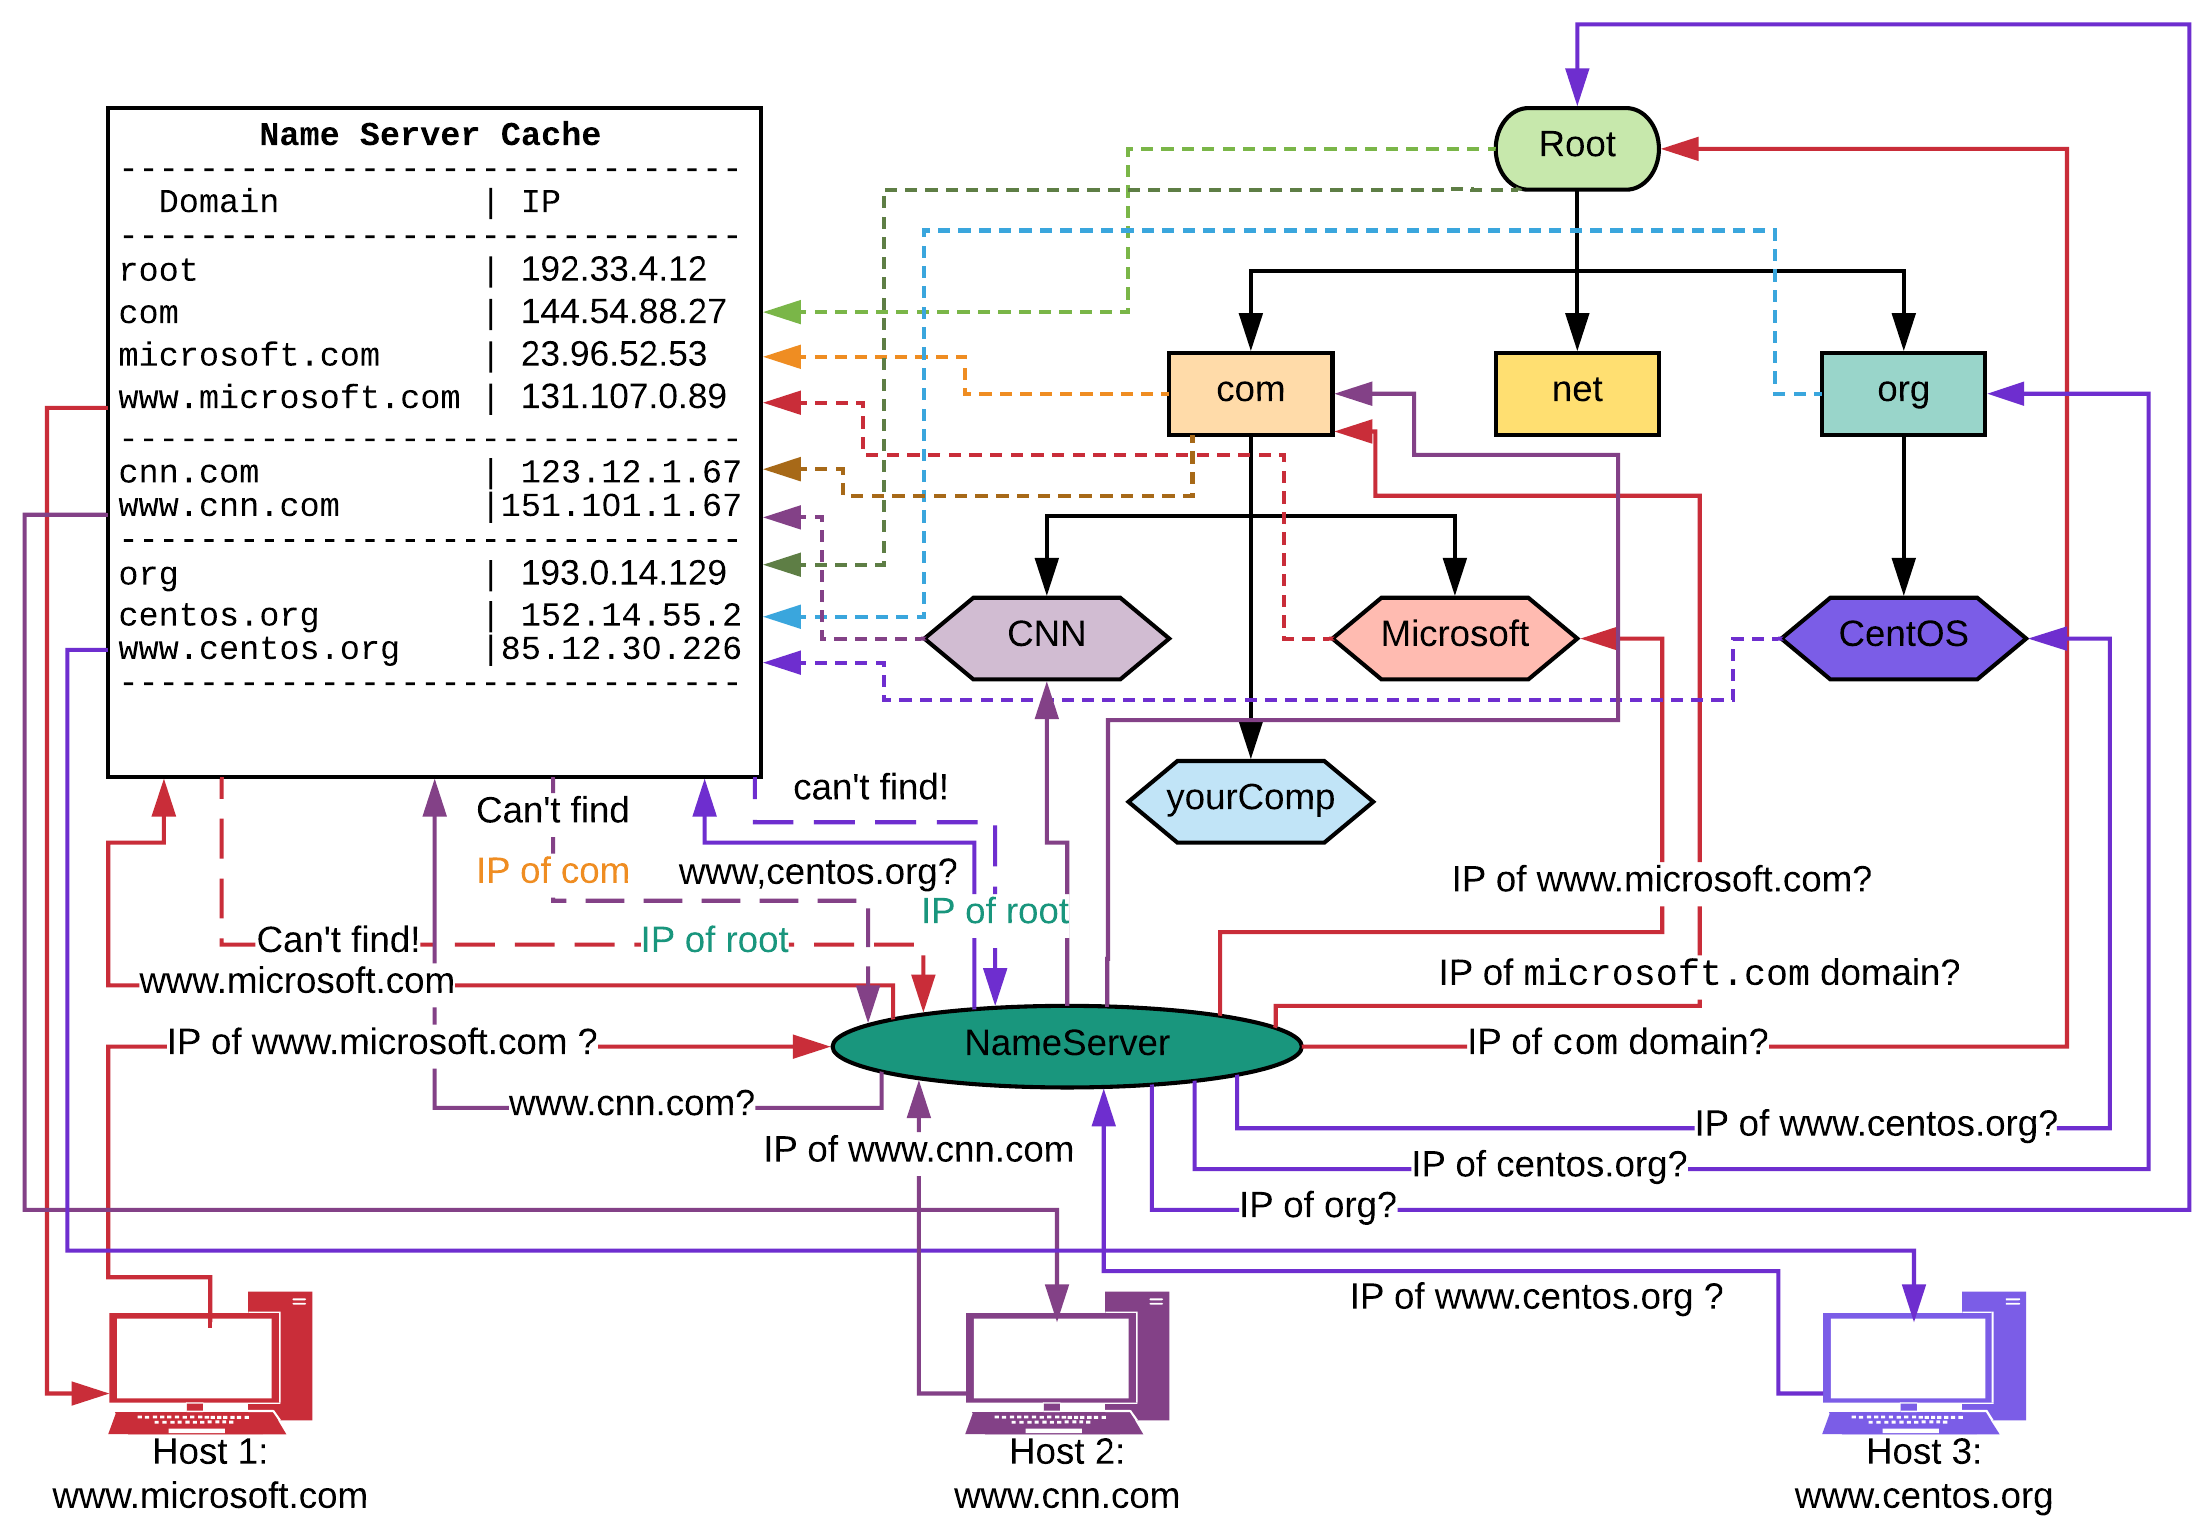
\includegraphics[width=1\linewidth]{Mod3/chapters/3.10.a}
	\caption{DNS Query with Caching}
	\label{fig:3}
\end{figure}

So now the DNS server has to perform \textit{recursion}, where it breaks down each part of the domain and gets an IP for each starting from the TLD till the IP of the original domain is found, while storing the IP for each domain in its cache. So, since the top level domain name is \verb|com| in \verb|www.microsoft.com|, it queries the root name server for the IP address of the \verb|com| domain. The reply is logged in the cache, and then the query for \verb|microsoft.com| domain IP is made to the \verb|com| name server. Again, the IP is logged and then a final query for \verb|www.microsoft.com| is made to the microsoft name server. When the reply is received, first the result is logged in the cache, and then the local name server realizes that this is the required IP that was queried by \textit{Host 1} and provides the IP address to it.

Next time a query is made by Host 2 for \verb|www.cnn.com|. Since the name server already has the IP of \verb|com| domain cached (from the query for \verb|www.microsoft.com|), it directly asks it for the IP of \verb|cnn.com|. Once received and cached, it now asks cnn.com for the ip of \verb|www.cnn.com|, and caches the reply and sends it to \textit{Host 2}. 

However, when \verb|Host 3| makes a query for \verb|www.centos.org|, the local name server again has to make a query to the root name server, since it doesn't have the IP address for the \verb|org| domain in its cache. Now again, it continues recursion (requests the IP of \verb|centos.org| to \verb|org| nameserver and then the IP of \verb|www.centos.org| to the \verb|centos.org| nameserver) till it has the IP of \verb|www.centos.org| in its cache and then passes it on to \verb|Host 3|. 

While the process of recursion is effective in finding IPs for domain names, it takes several recursive lookups to find the IP of a single domain. Thus, caching is important since any previously accessed site's IP can be served within a fraction of the time as compared to recursive lookup. 

\subsection{DNS Forwarding}
The act of DNS forwarding is to ask our local name server to directly query another name server somewhere on the DNS hierarcy (for example, at the provider level) to increase efficiency. Then, if the domain is unknown to the name server, then that name server will perform the lookup and present a reply, which our name server will then cache and present to the host that queried it. Thus, our name server has to do only one query!

\section{Understanding Different DNS Server Modes}
\subsection{Types of Nameservers}
\subsubsection{Primary (Master) Nameserver}
\vspace{-10pt}
A primary name server is responsible for a \textbf{zone}. A zone is the total collection of resource records within a domain and all sub-domains within it. 

\subsubsection{Secondary (slave) Nameserver}
\vspace{-10pt}
A secondary nameserver serves as a read-only backup nameserver normally. 

\subsubsection{Cache-only Nameserver}
\vspace{-10pt}
In a cache-only nameserver, only a cache of domain name lookups is stored and it doesn't store any resource records itself!

\subsection{Resource Records}
A resource record is used to store some kind of information about a domain name. Some types of resource records are:

\noindent
\begin{tabular}{rM{0.85}}
	\toprule
	\textbf{Terms} &\textbf{Description} \\
	\midrule
	\textbf{A}	&Resolves a domain name to an IPv4 address.\\
	\textbf{AAAA}	&Resolves a domain name to an IPv6 address.\\
	\textbf{CNAME}	&Canonical name or alias of a FQDN.\\
	\textbf{PTR}	&Pointer Records - Used for Reverse DNS resolution, i.e., finding a FQDN for an IP\\
	\textbf{NS}	&NameServer - identifies all name servers that are authoritative.\\
	\textbf{SOA} &Start of Authority - provides generic information about a domain\\
	\textbf{MX}	&Mail eXchange that is responsible for this domain - used to indentify mail servers on the internet.\\
	\textbf{TXT} &Used to supply additional data - such as data used by Sender Policy Framework (in email) networks. This particular one is used to verify the authenticity of the sender of the mail. \\ 
	\textbf{SRV} &Hosts that provide a specific service. \\
	\bottomrule
\end{tabular}

	\section{Analysing DNS output with dig}
To verify that our cache-only name server is doing its job properly, we need to verify that the DNS server is caching records. To confirm this, we use the \verb|dig| tool. If we use dig to look up the address of \verb|www.SomuSysAdmin.com|, we get:

\vspace{-15pt}
\begin{minted}{console}
# dig www.somusysadmin.com
; <<>> DiG 9.11.2-P1-RedHat-9.11.2-1.P1.fc27 <<>> www.somusysadmin.com
;; global options: +cmd
;; Got answer:
;; ->>HEADER<<- opcode: QUERY, status: NOERROR, id: 35715
;; flags: qr rd ra; QUERY: 1, ANSWER: 2, AUTHORITY: 13, ADDITIONAL: 12

;; QUESTION SECTION:
;www.somusysadmin.com.		IN	A

;; ANSWER SECTION:
www.somusysadmin.com.	174	IN	A	104.27.136.245
www.somusysadmin.com.	174	IN	A	104.27.137.245

;; AUTHORITY SECTION:
.			58786	IN	NS	j.root-servers.net.
.			58786	IN	NS	k.root-servers.net.
.			58786	IN	NS	l.root-servers.net.
.			58786	IN	NS	m.root-servers.net.
.			58786	IN	NS	a.root-servers.net.
.			58786	IN	NS	b.root-servers.net.
.			58786	IN	NS	c.root-servers.net.
.			58786	IN	NS	d.root-servers.net.
.			58786	IN	NS	e.root-servers.net.
.			58786	IN	NS	f.root-servers.net.
.			58786	IN	NS	g.root-servers.net.
.			58786	IN	NS	h.root-servers.net.
.			58786	IN	NS	i.root-servers.net.

;; ADDITIONAL SECTION:
j.root-servers.net.	38832	IN	A	192.58.128.30
k.root-servers.net.	174213	IN	A	193.0.14.129
l.root-servers.net.	30272	IN	A	199.7.83.42
m.root-servers.net.	210057	IN	A	202.12.27.33
a.root-servers.net.	192881	IN	A	198.41.0.4
b.root-servers.net.	87215	IN	A	199.9.14.201
c.root-servers.net.	68790	IN	A	192.33.4.12
e.root-servers.net.	86889	IN	A	192.203.230.10
f.root-servers.net.	223796	IN	A	192.5.5.241
g.root-servers.net.	199280	IN	A	192.112.36.4
h.root-servers.net.	159574	IN	A	198.97.190.53
i.root-servers.net.	2360	IN	A	192.36.148.17

;; Query time: 11 msec
;; SERVER: 10.10.70.1#53(10.10.70.1)
;; WHEN: Fri Mar 09 20:53:12 IST 2018
;; MSG SIZE  rcvd: 473
\end{minted}
\vspace{-10pt}	

\noindent
Thus, we can see the answer to the query was provided with two A records: which indicate the IPs: \verb|104.27.136.245| and \verb|104.27.137.245| point to the site. 

\subsection{Looking up specific Resource Records using dig}
The dig utility allows us to look up any type of resource record just by passing the name as an argument. To view the MX records for the domain, we use:

\vspace{-15pt}
\begin{minted}{console}
# dig MX somusysadmin.com
; <<>> DiG 9.9.4-RedHat-9.9.4-51.el7_4.2 <<>> MX somusysadmin.com
;; global options: +cmd
;; Got answer:
;; ->>HEADER<<- opcode: QUERY, status: NOERROR, id: 16995
;; flags: qr rd ra; QUERY: 1, ANSWER: 5, AUTHORITY: 13, ADDITIONAL: 7

;; QUESTION SECTION:
;somusysadmin.com.		IN	MX

;; ANSWER SECTION:
somusysadmin.com.	5	IN	MX	15 eforward4.registrar-servers.com.
somusysadmin.com.	5	IN	MX	10 eforward3.registrar-servers.com.
somusysadmin.com.	5	IN	MX	20 eforward5.registrar-servers.com.
somusysadmin.com.	5	IN	MX	10 eforward1.registrar-servers.com.
somusysadmin.com.	5	IN	MX	10 eforward2.registrar-servers.com.
...
\end{minted}
\vspace{-10pt}	

\noindent
The numbers after \verb|MX| in the answers section are the priority, with a lower number having higher priority. To view the \textbf{authoritative nameservers} for \verb|somusysadmin.com|, we use: 

\vspace{-15pt}
\begin{minted}{console}
# dig NS somusysadmin.com
; <<>> DiG 9.9.4-RedHat-9.9.4-51.el7_4.2 <<>> NS somusysadmin.com
;; global options: +cmd
;; Got answer:
;; ->>HEADER<<- opcode: QUERY, status: NOERROR, id: 41236
;; flags: qr rd ra; QUERY: 1, ANSWER: 2, AUTHORITY: 2, ADDITIONAL: 0

;; QUESTION SECTION:
;somusysadmin.com.		IN	NS

;; ANSWER SECTION:
somusysadmin.com.	5	IN	NS	fiona.ns.cloudflare.com.
somusysadmin.com.	5	IN	NS	guy.ns.cloudflare.com.

;; AUTHORITY SECTION:
somusysadmin.com.	5	IN	NS	guy.ns.cloudflare.com.
somusysadmin.com.	5	IN	NS	fiona.ns.cloudflare.com.

;; Query time: 318 msec
;; SERVER: 10.0.99.2#53(10.0.99.2)
;; WHEN: Fri Mar 09 21:04:56 IST 2018
;; MSG SIZE  rcvd: 114
\end{minted}
\vspace{-10pt}	

\subsection{Performing Reverse DNS lookup}
To perform a reverse DNS lookup, i.e., get a domain name for a given IP address, we use \verb|dig -x|:

\vspace{-15pt}
\begin{minted}{console}
# dig -x 8.8.8.8
; <<>> DiG 9.9.4-RedHat-9.9.4-51.el7_4.2 <<>> -x 8.8.8.8
;; global options: +cmd
;; Got answer:
;; ->>HEADER<<- opcode: QUERY, status: NOERROR, id: 53132
;; flags: qr rd ra; QUERY: 1, ANSWER: 1, AUTHORITY: 13, ADDITIONAL: 12

;; QUESTION SECTION:
;8.8.8.8.in-addr.arpa.		IN	PTR

;; ANSWER SECTION:
8.8.8.8.in-addr.arpa.	5	IN	PTR	google-public-dns-a.google.com.
...
\end{minted}
\vspace{-10pt}	

\subsection{Status of dig}
In everyone of the queries above, we had a self-explanatory \textit{NOERROR} status. However, if we try to lookup a FQDN that doesn't exist, then we get:

\vspace{-15pt}
\begin{minted}{console}
# dig doesnotxist

; <<>> DiG 9.11.2-P1-RedHat-9.11.2-1.P1.fc27 <<>> doesnotxist
;; global options: +cmd
;; Got answer:
;; ->>HEADER<<- opcode: QUERY, status: NXDOMAIN, id: 44834
;; flags: qr rd ra; QUERY: 1, ANSWER: 0, AUTHORITY: 0, ADDITIONAL: 0

;; QUESTION SECTION:
;doesnotxist.			IN	A

;; Query time: 46 msec
;; SERVER: 10.10.70.1#53(10.10.70.1)
;; WHEN: Fri Mar 09 21:13:22 IST 2018
;; MSG SIZE  rcvd: 29
\end{minted}
\vspace{-10pt}	

\noindent
The status of \textit{NXDOMAIN} stands for non-existent domain. This is typically due to user error. A status of \textit{SERVFAIL} would indicate server failure, which shows that something is wrong at the server level, like authentication in DNSSEC (Domain Name System Security Extensions) that hasn't been properly set up. 

	\section{Setting up a Cache-Only DNS Server}
In RHEL 7 the default cache-only name server is provided in the \verb|unbound| package. We can prepare it for operation by:

\vspace{-15pt}
\begin{minted}{console}
# yum -y install unbound
# systemctl enable unbound; systemctl start unbound
\end{minted}
\vspace{-10pt}	

\noindent
Starting the server doesn't make much sense yet since the configuration hasn't been done yet. The primary configuration for this DNS server is \verb|/etc/unbound/unbound.conf|. The first thing that needs to be configured is the interface. We can have it listen on all ports of all connected interfaces by un-commenting the line:

\vspace{-15pt}
\begin{minted}{lighttpd}
interface: 0.0.0.0
\end{minted}
\vspace{-10pt}	

\noindent
There is also an access-control parameter that decides which IP addresses can make recursive queries to the nameserver. We can allow everybody to do this by un-commenting the \verb|access-control: 0.0.0.0/0 refuse| line, and modifying it to:

\vspace{-15pt}
\begin{minted}{lighttpd}
access-control: 0.0.0.0/0 allow
\end{minted}
\vspace{-10pt}	

\noindent
Now since \verb|unbound| has no capability to store resource records, it needs a DNS forwarding address to perform lookups for addresses it can't find. For this, we need to define a \textit{forward-zone} for root in the DNS hierarcy, denoted by '\verb|.|' character. The forward-zone will then look like:

\vspace{-15pt}
\begin{minted}{lighttpd}
forward-zone:
name: "."
forward-addr: 8.8.8.8
\end{minted}
\vspace{-10pt}	

\noindent
We're using Google's DNS servers for DNS forwarding. This concludes our basic configuration. Unbound provides an easy utility to check for any syntax errors in our configuration, which we can use by:

\vspace{-15pt}
\begin{minted}{console}
# unbound-checkconf
unbound-checkconf: no errors in /etc/unbound/unbound.conf
\end{minted}
\vspace{-10pt}	

\noindent
Since we didn't find any errors in our configuration, we can now restart the DNS server and check that the service is running:

\vspace{-15pt}
\begin{minted}{console}
# systemctl restart unbound; systemctl status -l unbound
● unbound.service - Unbound recursive Domain Name Server
   Loaded: loaded (/usr/lib/systemd/system/unbound.service; enabled; vendor preset: disabled)
   Active: active (running) since Fri 2018-03-09 23:34:02 IST; 1min 7s ago
  Process: 5732 ExecStartPre=/usr/sbin/unbound-anchor -a /var/lib/unbound/root.key -c /etc/unbound/icannbundle.pem (code=exited, status=0/SUCCESS)
  Process: 5728 ExecStartPre=/usr/sbin/unbound-checkconf (code=exited, status=0/SUCCESS)
 Main PID: 5736 (unbound)
   CGroup: /system.slice/unbound.service
           └─5736 /usr/sbin/unbound -d
\end{minted}	 

	\section{Opening the Firewall for DNS}
The firewall needs to be configured to open port 53 for DNS. We can do this using:

\vspace{-15pt}
\begin{minted}{console}
# firewall-cmd --permanent --add-service=dns 
success
# firewall-cmd --reload
success
# firewall-cmd --list-services 
ssh dhcpv6-client http https dns
\end{minted}
\vspace{-10pt}	

\noindent
We can then confirm that the ports are open and unbound is listening on them using:

\vspace{-15pt}
\begin{minted}{console}
# netstat -tulpn | grep unbound
tcp        0      0 0.0.0.0:53      0.0.0.0:*       LISTEN     5736/unbound        
tcp        0      0 127.0.0.1:8953  0.0.0.0:*       LISTEN     5736/unbound        
tcp6       0      0 ::1:8953        :::*            LISTEN     5736/unbound        
udp        0      0 0.0.0.0:53      0.0.0.0:*                  5736/unbound 
\end{minted}
\vspace{-10pt}	

	\section{Working with Cache Dumps}
Sometimes we'll need to troubleshoot the unbound server for problems such as the cached data expiring. A straight forward solution to this is dumping and cleaning up the cache. 

\vspace{-15pt}
\begin{minted}{console}
# unbound-control dump_cache > dnsCacheFile
# unbound-control dump_cache | grep cnn
www.cnn.com.	0	IN	CNAME	turner-tls.map.fastly.net.
# unbound-control flush www.cnn.com
ok
# unbound-control dump_cache | grep cnn
#
\end{minted}
\vspace{-10pt}	

\noindent
So, by using the \verb|flush| command of \verb|unbound-control|, we can expunge the data about a certain domain name immediately, and the next time someone demands the data for \verb|www.cnn.com|, fresh data will be imported into the cache after a new DNS query. 

To replace the current contents of the cache with that of a cache file, we can use the \verb|load_cache| sub-command, which reads data from \textit{stdin}:

\vspace{-15pt}
\begin{minted}{console}
# echo dnsCacheFile | unbound-control load_cache
\end{minted}

\subsection{Fixing issues with no replies}
Sometimes, it may so happen that the cache-only DNS server doesn't reply with the necessary information, and reports that the "hostname wasn't found" or other such error messages typically signifying network issues. In such cases, the first thing to try is pinging google's name server at the ip address 8.8.8.8 (or any external IP that's not a private IP). If the ping is successful, it'll confirm an issue with the DNS server's settings. 

The next point is to check the logs. The location of the logs can be set manually in \verb|unbound.conf|, but generally it writes to the syslog. Thus, we need to check if there are any errors in it by:

\vspace{-15pt}
\begin{minted}{console}
# less /var/log/messages | grep unbound
\end{minted}
\vspace{-10pt}	

\noindent
If there are messages indicating: \verb|failed to prime trust anchor -- DNSKEY rrset |\\ \verb|is not secure . DNSKEY IN| and/or \verb|validation failure google.com. A IN| (after pinging google.com), then the issue is with the DNSSEC configuration. Since we haven't set it up yet, we can simply set it to permissive mode where even though the DNS server won't trust the replies that aren't validated, they'll still be allowed in the cache and be sent as replies to the client. For this, in \verb|/etc/unbound/unbound.conf|, we simply need to change the line:

\vspace{-15pt}
\begin{minted}{lighttpd}
val-permissive-mode: yes
\end{minted}
\vspace{-10pt}	

\noindent
This line is present in the \verb|server:| section of the config. Now, the server should be working properly!

